\section{Experimental setup}\label{sec:setup}
In chapter \ref{sec:theory} was explained the spontaneous parametric downconversion. This effect is used as a source of two entangled photons in this experiment. The experimental setup is shown in figure \ref{fig:setup}. As a nonlinear material a Beta Barium Borate (BBO) crystal is used. Then the two emmited photons have to pass polarizer to measure the polarization.  The last step is the detections of the photons with two single photons counting modules.
To improve the quality of the measured results filters like bandpass filters are used.
\begin{figure}[H]
\centering
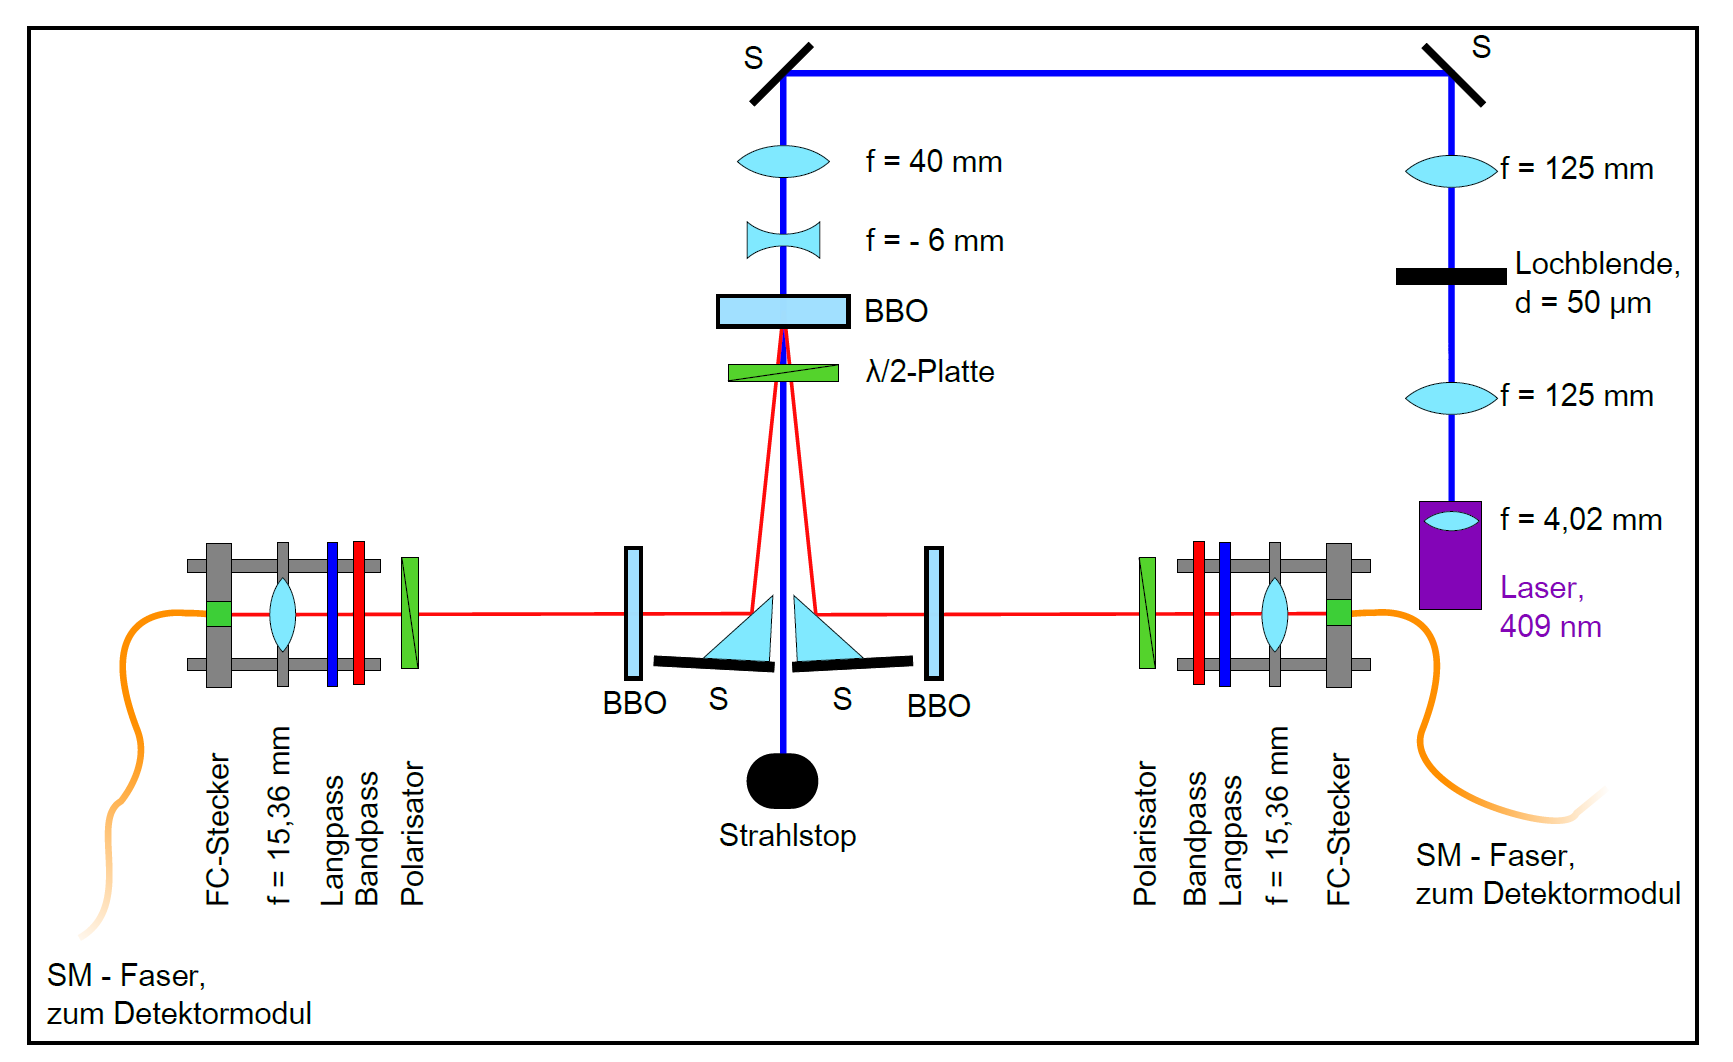
\includegraphics[scale=0.2]{figures/setup.PNG}
\caption{Scetch of the experimental setup to measure the polarization of two entangled photons to violate the CHSH-inequality \cite{barz}.   }
\label{fig:setup}
\end{figure}


The both entangled photons have a different polarization. That means they see different refractive indices during the propagation in the BBO crystal. There have to be a compensation of these effects which are called longitudinal walk-off and transversal walk-off.
The longitudinal walk-off effect describes the different velocities of the photons in the crystal, due to the different refractive indices for different polarizations. To compensate that, a half wave plate and a second BBO crystal is necessary. A scetch of the compensation is shown in figure \ref{fig:walk_off_longitudinal}. Dependent on the position in the BBO crystal where the parametric downconversion is happening, the photons have differen distances in the crystal. Because of the different velocities there is a time difference between the two photons when they left the crystal.   


\begin{figure}[H]
\centering
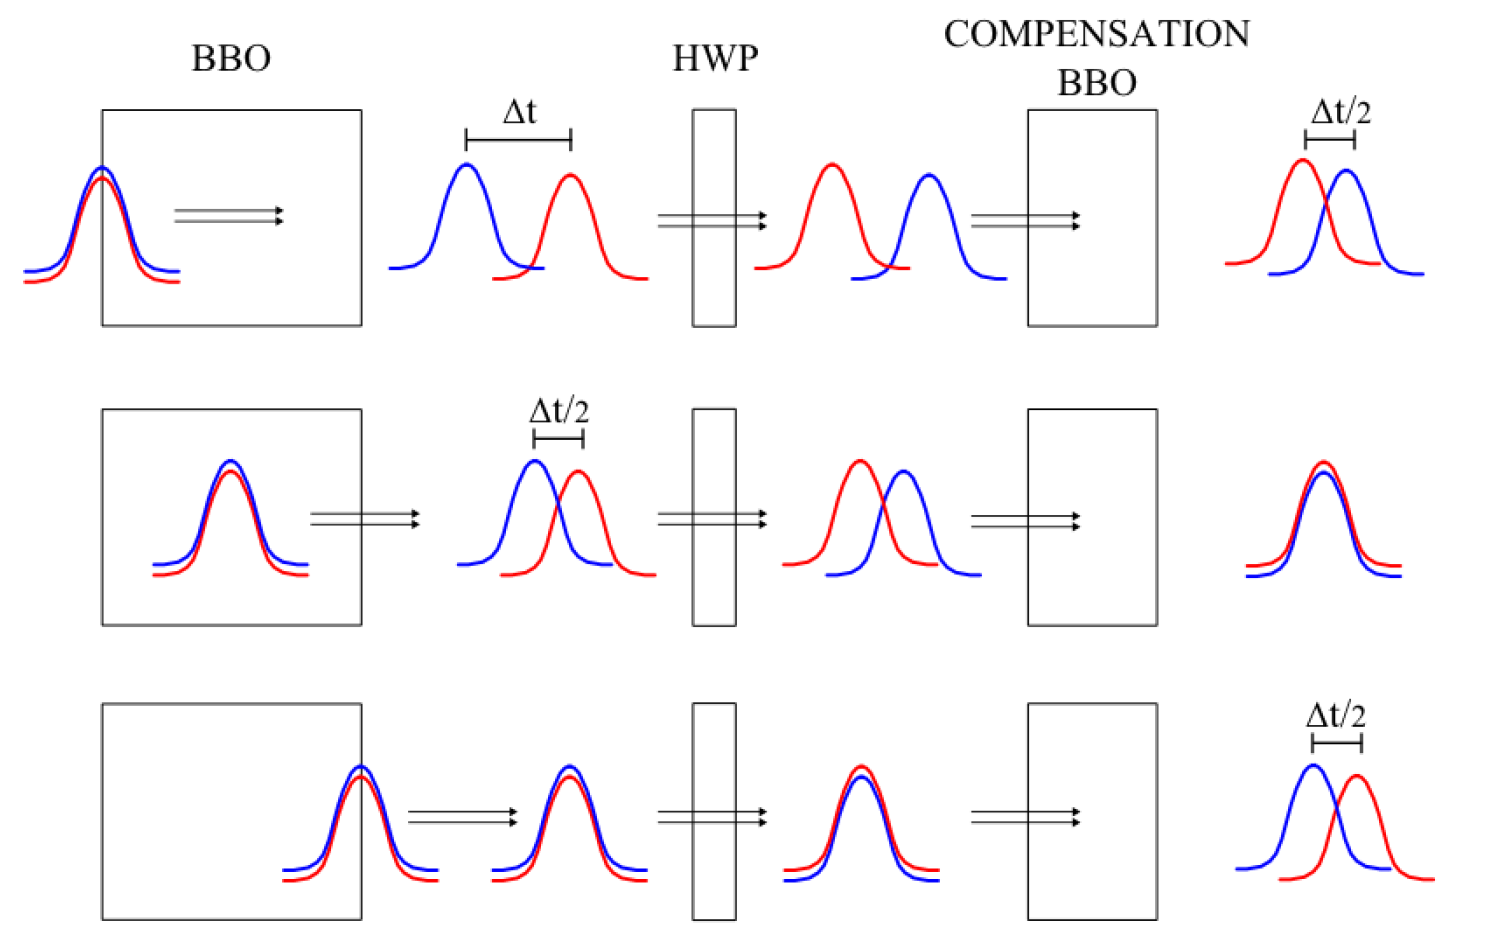
\includegraphics[scale=0.2]{figures/walk_off_longitudinal.PNG}
\caption{Scetch of the compensation of the longitudinal walk-off effect. Dependent on the position of creating the photon pairs, there is a time delay $\Delta t$. By using a half wave plate and a second BBO crystal, the time delay can be reduced to $\frac{\Delta t}{2}$ \cite{fimpel}.   }
\label{fig:walk_off_longitudinal}
\end{figure}
The tranversal walk-off effect describes the geometrical displacement of the extraordinary polarised photon in the crystal, as shown in figure \ref{fig:walk_off_transversal}. Analog to the longitudinal walk-off effect, the problem is that the photon pairs can be created everywhere in the crystal. The both photons are smeared out in the crystal. To compensate that can be used similarly to the longitudinal walk-off effect a half wave plate and a second BBO crystal.
\begin{figure}[H]
\centering
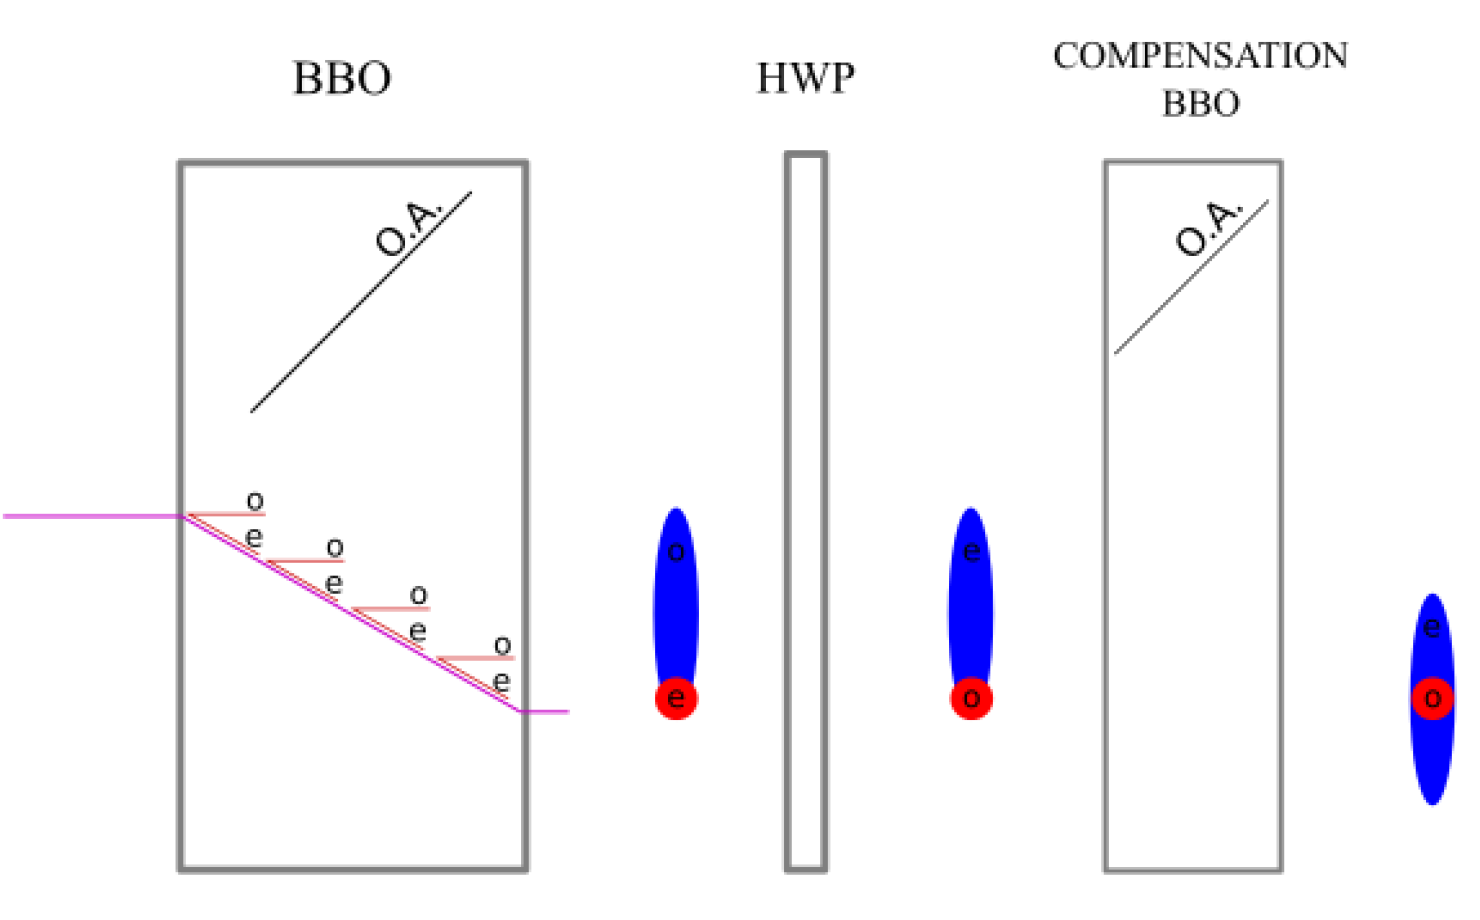
\includegraphics[scale=0.2]{figures/walk_off_transversal.PNG}
\caption{Scetch of the comopensation of the transversal walk-off effect \cite{fimpel}.   }
\label{fig:walk_off_transversal}
\end{figure}
